\chapter{Implementation}

This chapter describes the implementation of the features that were identified in the analysis. I will focus on the interesting parts of the implementation.

From a higher-level perspective, there are several subparts of the project that need to cooperate for the client app to work well. Firstly, there are the domain objects and stores implemented with the help of MobX. Secondly, there is the view layer created with React Native. The third piece is handling API communication and lastly, there are the native modules for handling job upload (ie. uploading files to Memsource and creating jobs from them) which are the only custom code of the application that is not written in JavaScript. Native code is also needed for the case when the Memsource application is opened from eg. the Mail application for job import. This chapter explains in depth the solutions to these tasks and issues encountered along the way.


In the following text, I will use the terms Javascript (JS) layer, native layer and asynchronous bridge. When talking about the Javascript layer, I refer to the Javascript code which runs in JavascriptCore engine. By native layer I mean the code that is being executed in the Android or iOS runtime environments. To explain the importance of these terms, let us quickly take a look at an example of how these affects us.

When React Native (RN) communicates between the Javascript and native layers, it uses batched messages that it sends through the asynchronous bridge. This means that if you want (or are forced to, in some cases) to access some value synchronously from one layer or another, it has to be available in that particular layer. In some cases this means a value has to be duplicated on both sides of the bridge and has to be synchronized using a call through the bridge. However, when a value exists on both sides of the bridge, we need some mechanism that will be able to determine which of the two values is the most-up-to-date one. 

As an example, let us consider the TextInput component (a text field) on iOS. Because of the design of the platform, the value entered in the text field  has to live in UIKit. We would, however, like to be able to control and read the text input’s value from Javascript synchronously. Imagine a text field into which we start typing “ABC” as input. At time 1, the native UI thread sends the first letter "A" to the JS thread. The JS thread, however, does not pick up the value until it is picked up from the event loop queue. At time 2, user enters "B" and the UI thread sends the value “AB” to the JS queue. At the same time, the text field value is set to “A” in response to the update sent from the JS thread. At time 3, user enters "C" and so the UI thread sends “AC” to the JS queue. At the same time the value “AB” that JS just received is sent through the bridge to the native layer. In the end, the JS thread receives “AC” and sends it again through the bridge. Both the native and JavaScript layers now contain the same value - “AC” but the character “B” has been dropped! The solution implemented in RN involves a counter of input events of the text field which is sent through the bridge and the value of the text field is not changed unless the counter number received from JS is higher than the one stored in the native layer.

This gives us understanding of the Javascript layer, native layer and the asynchronous bridge. This also explains some unexpected effects that a developer may meet when working with native UI controls.


\begin{figure}
	\begin{forest}
		for tree={
			font=\ttfamily,
			grow'=0,
			child anchor=west,
			parent anchor=south,
			anchor=west,
			calign=first,
			inner xsep=7pt,
			edge path={
				\noexpand\path [draw, \forestoption{edge}]
				(!u.south west) +(7.5pt,0) |- (.child anchor) pic {folder} \forestoption{edge label};
			},
			% style for your file node 
			file/.style={edge path={\noexpand\path [draw, \forestoption{edge}]
					(!u.south west) +(7.5pt,0) |- (.child anchor) \forestoption{edge label};},
				inner xsep=2pt,font=\small\ttfamily
			},
			before typesetting nodes={
				if n=1
				{insert before={[,phantom]}}
				{}
			},
			fit=band,
			before computing xy={l=15pt},
		}  
		[js
		[app.js,file
		]
		[api
		]
		[components
		[formComponents
		]
		[jobs
		]
		[projects
		]
		[translationMemories
		]
		]
		[flow
		]
		[global
		]
		[models
		]
		[stores
		]
		[utils
		]
		]
	\end{forest}
	\caption{Simplified folder structure of the project.}
	\label{impl:folders}
\end{figure}

Figure \ref{impl:folders} shows simplified schema of the project structure. Since React Native makes no assumptions about the rest of the development stack, developer has the freedom to structure the project as they find fit. In my case, I first created dedicated folders for domain objects (models) and stores. All components live in the \texttt{components} directory which is further divided based on where in the application the components are used or what purpose they serve. The \texttt{api} folder contains the objects related to connectivity and communication with Memsource API and the remaining folders provide supporting utilities such as global styles. Native code and modules are placed higher in the directory structure so they are not visible in the figure.


\section{UI with React Components}

User interfaces made with React consist of components, which are independent and reusable pieces of code. The complete application UI consists of a tree of components. In the case of this project, the root component is defined in \texttt{app.js} in the \texttt{js} directory as can be seen in figure \ref{impl:folders}.

The main way of modifying component behavior is composition - by wrapping a component and adding some functionality, we create a new one. Since the app needs to support lots of CRUD operations we need components for choosing date, choosing one or more items from a small as well as large lists and more. One of the first issues I have encountered is that finding form components which would look according to what is customary on both platforms is hard. While there are UI toolkits for React Native such as Shoutem UI Toolkit or NativeBase and community-developed components, none of them offered quite the functionality that I needed at the time when I evaluated them.

I therefore created wrappers around the basic form components provided by React Native and gave them default styling which is overridable (for example a label or an icon can be added) and mode (for example modal or inline pickers on iOS). All of these options are available under a unified interface of the component, which allows it to be easily used throughout the app. The figure shows an example of different look of ListPicker and DatePicker components on Android and iOS. Note that the pickers on iOS can be displayed both inline and in a modal at the bottom of the screen. Android ListPicker on the other hand, can be displayed in a dialog or as a dropdown.

\begin{figure}[H]
	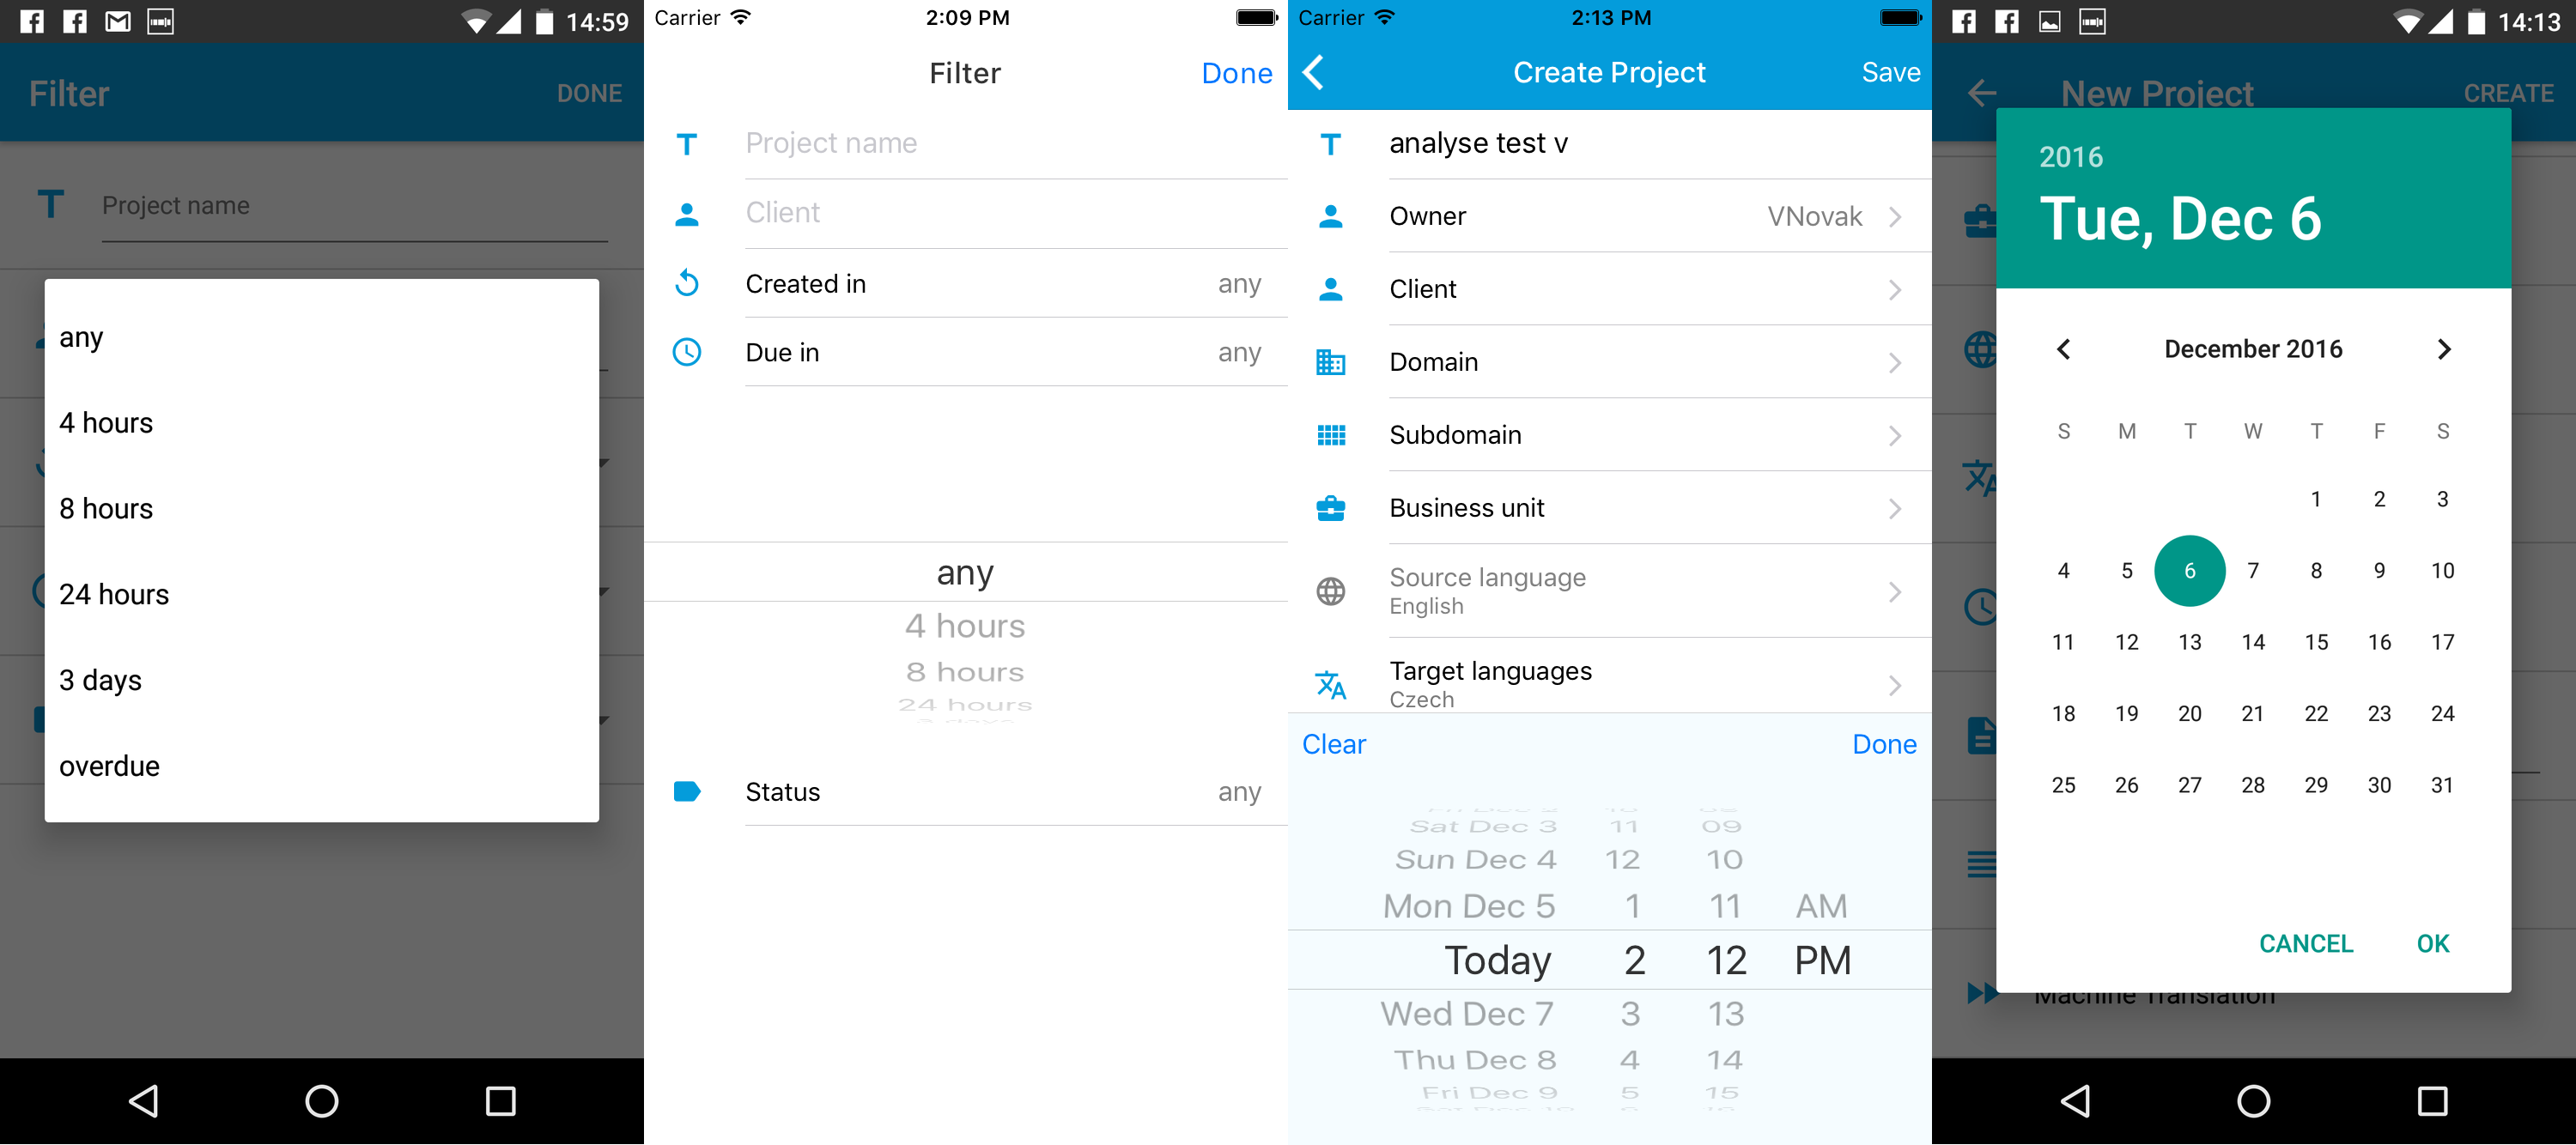
\includegraphics[width=1\textwidth]{pics/components}
	\caption{Platform-customized behavior of list and date picker components}
	\label{components}
\end{figure}


When using such components in code, one only has to provide them with the information about the icon, the values they need to show, the mode and how they should respond to user action. The logic of how the component should be displayed and styled is hidden inside of it, with the styling being overridable. This way we can construct reusable components with platform-specific behavior. This, in my opinion is a very powerful concept, since as the community evolves it will create components that serve the same purpose and have the same interface, but may look even completely different per platform. The code responsible for the different behavior, however, will be hidden inside those libraries and we will just plug the components into our projects. This will allow to focus more on the business logic of the app while enabling to develop it so that looks as is customary for the platform it runs on.


%As described in the todo section, React native offers several ways of how to handle per-platform customizations. We will use these to provide user with the app handling they are accustomed to. Examples of places that need custom handling are actions that are included in the navbar on Android while they're shown in the bottom toolbar on iOS. Also the navigation has to look differently. 

\section{Stores}

As explained in section \ref{sec:stores}, the information about projects, jobs, and other entities in stored in domain objects, which in turn are kept in stores. It is important that there is always only one instance of a particular domain object in memory, and only one instance of a store.

As an example of how a store is implemented, let's consider the project store whose class diagram is in figure \ref{projectStore} on page \pageref{projectStore}. In its constructor it accepts (among other) the user store - that way we can reactively clean and refresh the project list in case the active user changes. This is done through the aforementioned autorun function from MobX. It also receives ApiCaller instance which is used for communication with Memsource API. Projects are stored in a Map data structure, which is typically backed by a hash table that offers constant access time, or by other mechanism that provides sublinear access time \cite{ecma:map}. The keys of the Map are projects ids and the values are instances of Project class. That way we can access the stored project instances quickly, which is especially convenient because the projects are displayed in multiple tabs that correspond to filters in Memsource Cloud (all, in progress, overdue, my). One project may be displayed in any number of tabs and even when a project is displayed in all four of them, internally this refers to the same project instance. Also, when the app receives a JSON (JavaScript Object Notation) containing projects, it can quickly see whether or not a project is already stored.


\subsection{Connecting Stores with Views}

Clearly, stores need to be made available to React, so that components can visualize the content of the domain objects. For this purpose, the mobx-react package offers the \texttt{Provider} component and \texttt{@inject} decorator, thanks to which arbitrary objects can be passed to React components as props. Internally this uses React's context to function.

As I explained earlier, React app is composed of a tree of components where props are passed from top to bottom. You can either pass the stores as props explicitly through the entire tree which can get tedious, or use \texttt{Provider}, and grant store access for them by using inject. This makes it simple and transparent to "connect" components with relevant parts of the state. Listing \ref{code:provider} shows a simple example of how color prop can be injected. We can still pass the prop explicitly from the parent component, in which case the explicit prop takes precedence. This can be taken advantage of in testing.

\lstinputlisting[label=code:provider,caption=Using MobX Provider and inject]{./code/provider.js}

I have used the \texttt{Provider} component extensively, but almost exclusively for the application's screens (e.g. job list screen) to get access to the stores, and for any components used within the screens, I pass the stores explicitly as a prop.


\section{Upload Module}
Upload module is a native module made to allow users to upload files to Memsource Cloud and create jobs from them. It offers different ways to select the files and allows to set up various import options. After the upload is triggered, a new item (a \textit{{temporary job}}) representing the ongoing upload is added to the job list. A notification and the network activity indicator on Android and on iOS, respectively, inform the user of the ongoing upload. 

There are important differences in the iOS and Android implementations, but both expose the same interfaces to the JavaScript layer. When talking about file handling in the native module, I will use the singular form for simplicity, but note the upload module has capabilities for uploading multiple files.



\subsection{Android}
To upload a file as a job, user has to either start the app and navigate to the “add job” screen and select the files for upload from a file picker, or start the app “externally” by opening a file using the Memsource app, for example from the Gmail app or a file browser. 
In both cases, the app receives a uri which points to the file. Note that the file doesn't necessarily need to be on the device, it may as well come from a cloud storage such as OneDrive or Google Drive. The user then sets up various options for the import and taps the “send” button. 
Upon pressing the button, the necessary information is passed to the upload module and upload is started. The information includes the following fields.

\begin{itemize}
	\item token
	\item upload url
	\item upload id
	\item project id
	\item user id
	\item whether the job should be pre-translated
	\item file information: uri, file name, id of temporary job
\end{itemize}


%At the same time, a new item is added to the job list. This item is displayed at the top of the list and, along with a notification, informs user of the running upload. http://wiki.memsource.com/wiki/Asynchronous_API_v2#Get_Asynchronous_Request


The module runs a background service whose responsibilities are issuing a notification when the upload starts, when the job is imported or if there was an error. The notification also shows different stages of the job creation - uploading of the file, file import and pre-translation, if selected. 

To upload a file, we first need to check whether it is present on the device. If not, file is downloaded. For working with the uri object, the service uses the Storage Access Framework API introduced in Android 4.4. The next step is uploading the file to Memsource and creating a job from it. This is done through  the \href{http://wiki.memsource.com/wiki/Job_Asynchronous_API_v2#Create_New_Job}{\texttt{Create New Job}} API call which handles the upload and puts the file into a queue where it waits for import. A server backend service dequeues the file and creates a job from it. Because dequeuing and job creation can potentially be long-running operations, the API call returns an ID of the enqueued object immediately after the upload is finished. The Android service then repeatedly polls the \href{http://wiki.memsource.com/wiki/Asynchronous_API_v2#Get_Asynchronous_Request}{\texttt{Get Asynchronous Request}} API to check if the job was already imported.

Once done, it issues a final notification or, if the user checked the pre-translation checkbox at job upload screen, continues with pre-translation based on project settings. This is another long-running operation and the native module keeps polling the \texttt{Asynchronous API} to check the pre-translation until it is confirmed. At that point it issues the final notification.


The service repeats its download and upload requests if there was an error and is also made to run in the background so that its actions are not disrupted in case the user switches to a different app or even “kills” the app by swiping it away from the screen. The upload service also stores the results of uploads in SharedPreferences so that if the application is killed and the job creation finishes in background, it can be updated the next time it starts. The token is not persisted.
If the app is still running in the foreground at the time when the job creation is confirmed, an event is sent to JavaScript and the views are updated. If that is not the case, the response of job creation is processed the next time the app is started or switched from background to foreground. If creation was successful the item (temporary job) which was previously added to the top of the job list is removed and the job list is re-fetched. In case of an error, the item is not removed but instead gives user an option to repeat the upload or remove the item manually. The native module is written in Java. 
 

\subsection{iOS}
On iOS, the module provides the same functionality but behaves very differently internally. iOS is much stricter about how background tasks are handled. There are fewer things that needs to be taken care of by the developer and more that are taken care of by iOS. This gives the developer a lot less flexibility (which also resulted in a problem with the API) but also results in less coding. The job creation on iOS works in the following way: similarly to Android, files can be selected within the app or sent to the app from an outside application such as Mail. If a file is selected using the Document Picker, iOS automatically downloads (if needed) and saves it to the app’s sandbox from where it is removed when the application exits. In case of importing the file from other application, the file is copied to app's sandbox and the application receives the url of the file. In the latter case, removing the file is the developer's responsibility.

Originally, I wanted to use the same approach for creating job as on Android, but it turned out not to be suitable because it is not possible to upload a file using the \texttt{multipart/form-data} request in the background. The reason it is not possible is that \texttt{multipart/form-data} needs to modify request body. A file uploaded by iOS's background upload task is sent directly in the body of the request and having a custom request body is impossible unless we write it directly into the file (which cannot be considered a good practice). Possible workaround here is to use another Memsource API, the File API which allows to upload a file in the request body and returns a file ID which can be used in other API calls. The problem with this approach is that we need to make two API calls to make the job import happen: first to upload the file and second to call the \texttt{Create Job} API. This poses a possible issue since iOS may decide to not perform our background request.

iOS uses several pieces of information to decide whether or not a request will be carried out. The decision involves eg. how of often the app is used by the phone's owner or what the battery level is. The exact algorithm is not publicly available. It may therefore happen that the first request for file upload will be honored but the second request for actually creating the job may be ignored. There is another situation when the call may not happen - if the application is awaken too often in response to its background requests, the interval in which it is be awaken will prolong, and again it may thus happen that the request for job import is carried out hours after the job was uploaded.

The best possible solution to this is implementing another API which would accept the file in the request body and the numerous parameters sent to the the \texttt{Create Job} API would be sent as a JSON string in a special request header. For the time being, I have implemented the described workaround and a better solution on the server side will be implemented later. 


Similarly to Android, as the upload starts, all of its information except the token is serialized and stored to UserPreferences entry and is updated whenever the status of the upload or import changes. This way the information is not lost when the app is killed during or after the import and the information about whether an upload was successful can be processed the next time the app starts or resumes: if the file was uploaded and import was requested on the server, the job import is considered successful an the  temporary job entry is removed from the job list. If the upload did not finish or if the import wasn't requested, the item is kept in the list and flagged it as a failed import. The iOS native module is written in Swift 3.


\section{State Persistence}

One of the implemented features is having parts of the app's data stored on the device so that it is available right after the app’s startup. This includes information related to projects, so that when the app starts, the user sees their projects immediately, along with a loading indicator which denotes that the projects are being refreshed. MobX itself doesn't come with a mechanism for state persistence, and therefore another library, Serializr was used. Serializr provides a variety of functions for serializing data stored in different data structures and also custom objects. The data that needs to be serialized and the data structure used are described using decorators placed on the member variables of selected classes. The application also stores search history for all of its users. 

While the implemented (de)serialization works well, it poses extra layer of complexity; implementing it was a lengthy task partly due to some hard-to-find unexpected behaviors and unhelpful error messages. The (de)serialization, however, is implemented in such way that when an error happens (which is more likely to happen during deserialization), the app falls back to to not deserializing any data and instead loads the data only from the API.


State is serialized upon switching the app into the background. The number of items that are serialized is limited so that the set of (de)serialized data doesn't grow indefinitely. Serializr outputs a JSON object which is persisted using React Native’s AsyncStorage as a string. Note that storage of user credentials is handled differently and is described in the next section. Upon app start, the objects that hold state are created empty, the JSON string is deserialized and and all of the information is inserted back into the state objects through setters. 


\subsection{Storing User Credentials}

Communication with the Memsource API requires the user to enter their username and password. The app then asks for a token which is used for the requests to follow. The token validity is limited to 24 hours and the app therefore needs to request a new one once the current token's validity is approaching its expiration date. To be able to ask for a new token, the app needs to have the user credentials at its disposal, and persist them so that it doesn't need to repeatedly ask the user to enter them. Such storage, obviously, needs to be safe and the AsyncStorage used for state persistence does not meet the safety criteria. To store the user credentials, I used a package which internally uses Keychain on iOS and an encrypted SharedPreferences entry on Android. I authored the Android part of the package which is now available as react-native-keychain on npm. 

\section{Data Fetching}

Application fetches all data through the \href{http://wiki.memsource.com/wiki/Memsource_API#API_Reference}{''Memsource REST API''}. The data is provided in JSON which makes it easy to work with, given that the app is written in JavaScript. The API uses standard HTTP response codes to denote operation result and provides error description when a request is incorrect.

There are some common patterns related to data fetching arising throughout the app. In many places we need to display some data, be able to reload it (using the well known pull down gesture), and be able to load more of the content and append it to the existing data (informally known as infinite loading).

Many of the used APIs use paging, ie. they deliver results in batches of 50 items per request (or less if more aren't available). The app uses this fact to find out if more items can be fetched since the number of the next page to be fetched can be calculated as $next = number \;of\; received \;items / 50$. If a response contains less than 50 items we know there are no more items to be fetched. However, we need to keep in mind that items can be both added and removed to the lists, for example when projects are added or deleted. That would give us a page number which is not an integer. In that case we perform a request for a page whose number is the closest lower integer. This may give us items that are already stored in the list, in which case we remove items at indices from $next \cdot 50$ to the end. That way we display the correct data and do not need to make any additional requests.

Also, in some cases we want to limit the number of pages that we fetch so that we do not allow the app to keep too many objects in memory which could cause undesired behavior. 

In some places where data is fetched we want to give the user a possibility to refresh the loaded list (such as in project or job lists) while in other we only offer listing without refreshing. This means we need to control up to two loading indicators that will denote refreshing (that would be the pull down indicator) or loading more content (loading indicator at the bottom of a list). We also need a means for blocking a request if it is already in progress or if it is forbidden (because of reaching the limit of how many items can be fetched or because no more items are available). 

Blocking a request if it already in progress is needed for cases when we eg. scroll down a ListView which has the infinite loading implemented. Infinite loading is implemented using ListView’s \texttt{onEndReached} function. This function is invoked when a user scrolls down the ListView and arrives at some pre-defined distance from the end of its content. Invocation of this function triggers fetching more items. In case of a poor network connection, fetching might take several seconds during which the user may scroll through the already rendered items and trigger another fetch. We need to prevent this second fetch from happening, otherwise when the returned promise resolves, it would append the results to the end of the list two or more times, causing duplicate entries.
 
If we want to have some universal fetching mechanism, it needs to account for all of these requirements. For this purpose I implemented the ProjectDetailsFetcher module. The most important function it exposes is the fetchProjectDetail function which accepts a project for which it fetches the detail (jobs, translation memories and term bases or other items  potentially added in future). The other parameters include the field name (eg. jobs), a boolean denoting whether the request is a full reload request (one triggered by the pull down gesture), configuration object (eg. to specify a filter) and page limit that will not allow fetching more than specified number of pages.
ProjectDetailsFetcher internally handles the number of the next page that should be requested for a particular project and property as well as tracking which requests are allowed or not. The fetchProjectDetail function returns a Promise which contains the response data. This data is usually requested from stores. ProjectDetailsFetcher does not handle displaying or hiding the loading indicators, as I have found it to be better to control this from the places where fetching is being requested because it offers more flexibility.




\subsection{Handling Internet Connection Outage}

The application’s functionality is dependent on Internet connection since acquiring all of its data and possible user actions need access to the internet. However, once the application fetches its data, it, of course, stays in the memory and is available for reading. Moreover, the app serializes data which is needed to display the list of projects and the project info screen, which includes projects, clients, domains, subdomains, business units and other details. That way the data is available for reading even if the user starts the app without internet connection.

When the app is offline, there is a bar displayed at the top of the screen, which informs the user that there is no internet access. Also, when a user's request times out, they are informed about it via a toast. This behavior however, may change if it is found to be too intrusive.


\section{Multi-stage Deployment and Testing}


One of the advantages of using React Native or hybrid application frameworks is the ability to use services such as Code Push \footnote{https://microsoft.github.io/code-push/} that enable the developer to update the application without going through Apple AppStore or Google Play Store submission process. This is achieved through being able to switch the JavaScript bundle which contains the app’s logic for another one. When a developer wants to publish a new version of the app they create a new JavaScript bundle and upload it to a Code Push server. 
When a user starts the app, it downloads the new bundle (if available) and stores it. In a typical scenario, the bundle would be applied upon the next app start but this is configurable. This way the user receives updates without any interruption on their side. This does not only give us the ability to publish updates at an arbitrary frequency but also offers greater control over the updates, since the user does not influence them.


In the app, I have used the Code Push service which is being developed by Microsoft and currently offered free of charge. 


Other possibility this offers and that I have implemented is multi-stage deployment and testing. For the purposes of our app, three build configurations were set up: debug configuration where Code Push is not being used; this configuration is used for everyday development and runs in React Native’s Dev mode. In Dev mode, React Native reports warnings and errors to the developer directly on-screen and performance is decreased.

The second configuration is Staging, which is set up to request the staging version of the JavaScript bundle from Code Push and uses Memsource’s pre-release server at \texttt{cloud 9.memsource.com} to serve its requests. This version is made for testing the application's new features and also its compatibility with the Memsource Cloud version which is the next to be deployed to production. The development mode is not enabled in this configuration and thus the app behaves like a production application. 


Finally, the third setup is for release. This configuration uses the corresponding JavaScript bundle from Code Push to get its updates. This is the version that runs on the phones of the Memsource’s customers. When suitable, the updates made in the staging version can be easily promoted to the release build of the application by a single Code Push CLI (Command Line Interface) command.

\section{Code Quality Tools}

Due to JavaScript's dynamic nature and the absence of any transformation that would try to verify its correctness before it is run, it is relatively easy to introduce bugs that only come to light during runtime. There are, however, tools for code quality assurance that help developers find potential bugs before the code is executed. In this project, I have used two such tools which this section shortly describes.

\subsection{Flow - Static Type Checker}

Flow \index{Flowtype} \footnote{https://flowtype.org/} is a static type checker for JavaScript developed by Facebook. It works by using type inference on JavaScript code even without any additional information provided by the developer. It tracks the type of variables as they are used throughout a program and allows to catch bugs before it is executed, without changing the existing code. 

Flow attempts to infer the types whenever possible, but JavaScript code can be very dynamic and hard to analyze statically. Flow therefore offers ways to specify types explicitly.

Flow supports standard primitive types such as number or string, as well as custom types eg. for application-specific objects. It guards common bugs such as null dereferencing, silent type conversions and many more potential sources of bugs. An example of how flow-typed code can look like, see listing \ref{code:flow}. In this example, Flow would report that the annotated return type of \texttt{string} is incompatible with the return type of the \texttt{length} function, which is a \texttt{number}. The listing also shows how to enable Flow checking for a JavaScript module --- this is done by putting \texttt{@flow} in a comment at the top of the file.


\lstinputlisting[label=code:flow,caption=Flow-annotated JavaScript code]{./code/flow.js}



I have used Flow extensively throughout the project and annotated the code regularly, because apart from the type checking, the annotations works very well as documentation for the developer and also for an IDE which can offer a better autocomplete. One of features of Flow I found very useful are maybe types which are denoted by a question mark (eg. \texttt{?string}). When accessing a function or property on an object which is of maybe type, Flow will issue a warning that \texttt{Property cannot be accessed on possibly null or undefined value}. This greatly helps avoiding the "Undefined is not an object / function" error which is one of the most common ones in JavaScript development. Other handy features I have used include interfaces or guarding against a function receiving too few or too many parameters. My estimate, based on running \texttt{git grep} for several of the most common types, is that there are more than 700 Flow annotations placed in the app's files.

\subsection{ESLint}

ESLint \index{ESLint} \footnote{http://eslint.org/} is a linter -- a tool that flags potential problems in source code. ESLint takes the form of a set of rules that the developer specifies and ESLint warns her when the code violates a particular rule. Rules may describe a potential bug in source code (such as calling a function that is not defined) or a desired coding style (such as using semicolons at the end of a line).

ESLint itself does not force any rules onto the developer. Instead, different rule sets can be obtained online and plugged into the project. Choosing such rule set is often a matter of personal preference or the technology that the project uses. For example, there are React Native-specific rules that eg. warn about having unused style definitions in the component code. 

During development, I have used ESLint rules assembled by the React community, available on npm under eslint-plugin-react, eslint-plugin-react-native and eslint-plugin-flowtype.


\section{Navigation}

In the context of React Native, by navigation I mean transitioning between different screens of the app. Navigation integrates with the components and also stores very closely, because many parts of the code will want to trigger navigation a different component as a response to user input or network event, so the navigation solution is of great importance. 

React Native started off with two solutions for navigation - the Navigator and NavigatorIOS. Navigator is implemented entirely in JavaScript, runs on both platforms and tries to mimic the appearance of native navigation, while NavigatorIOS leverages the native navigation of iOS.
They originally started as two competing implementations solving the same problem \cite{rn:navigation}  with the goal of assessing which of the two solutions should be supported further on. Ultimately, the Navigator solution was found to be better for reasons described later on, and Facebook used it in the F8 and Facebook ads applications. 


There is one notable drawback to Navigator - it is only trying to mimic the native navigation. This includes navigation bar with its animations, as well as transitions to and from different scenes of the app and implementation of the swipe back gesture. This, to a certain extent, can negative affect the user experience.
Having navigation controlled by JavaScript has its benefits - most importantly it allows for complete control of the navigation state, while with NavigatorIOS, some information sent from JavaScript to the native layer gets stored in the native code where it is managed by iOS internally which makes it hard to keep the information in JavaScript up to date. The difficulty of keeping JavaScript in sync with iOS and the fact it only works on one platform were the main reasons why Facebook decided to favor the Navigator.

Some would say that not using the native navigation breaks the promise of React Native - that is to be able to create apps that are indistinguishable from native ones. This is why Wix (an Israeli mobile and web development company) is working on a native navigation for react native. At the time of writing, there is not a stable release of this package available which is why I didn't use it.

Over the course of time new issues with using Navigator emerged and there was a need to come up with a better way of managing the navigation state. For example, the original Navigator becomes hard to work with in case we use several instances of it. For example, the application I have developed uses three different navigation components - one StackNavigation as a root navigator. The root navigator contains another StackNavigation where the vast majority of the app's content is pushed. In some places, however, I wanted to display modal windows. The modals are pushed onto the master navigator so that they are displayed in the foreground. The modal window contains another StackNavigation of its own, which yields a total of three navigators, but for applications that use a tab-based navigation or drawer navigation, that number is very likely higher. 


At the time when I started working on the project, the new solution to navigation was already present in the RN core and was named NavigationExperimental. However, since NavigationExperimental is only a set of low-level components, people started writing libraries around them to provide a more feature-rich experience for the developers. In the end, I have settled with a library called ex-navigation. It offers some needed functionality out of the box and allows to customize the behavior for iOS and Android such as handling the navigation bar, animations and back gesture on iOS as well as the back button handling on Android. Most importantly it works well with several navigators which can be managed independently and offers better animation performance - on Android, the animations are controlled from the native layer.

\section{Issues}

There were a number of issues encountered throughout the development, caused by different factors such as React Native's immaturity and frequent releases where new version is shipped every other week and updating is not always straightforward due to breaking changes (although this is changing to one release per month as of January 2017), lack of quality documentation, or my effort to create partially different UIs on each platform so that the user experience is on par with what the user would get in an application designed specifically for iOS or Android. This sometimes led to dead ends such as when I had to replace the entire navigation solution for a new one. Navigation as a whole is an interesting topic, which is why I devoted an entire section to it.
Another issue is minor differences in behavior on each platform -- the component appearance on iOS may not always be the same as the one on Android. This involves borders, border radius or animations. However, given React Native's complexity --- the library uses JavaScript, Java, Objective-C, C++ and also C --- it does a very good job in abstracting the platform away.
Other very painful issue, although visible only when rendering large UIs, are animations which are controlled from the JavaScript thread. This means that the JavaScript thread has to periodically send commands to the native layer for the animation to run. If the JavaScript thread has too much work on it, issuing the command is delayed and the result is a laggy animation. This issue, however, is already partially solved and offloading the animations from the JavaScript thready will probably be fully functional in the first months of 2017.

Other difficulties were met in working with files (uploading and downloading jobs), since this needed to be done once for each platform and involved coding in Java as well as Objective C and Swift. Working with files has many hidden culprits given by different behavior on older Android versions, file permission issues and problems resulting from different file sources - ie. files imported from other applications vs form UIDocumentPicker on iOS.
%Also, the fact that React Native is not a framework gives developer the freedom to do things in different ways, which also means that the first way a developer reaches for does not always turn out to be the best one. 


\section{Open Source Software Contributions}

Throughout the development of the application, I have contributed to different projects by bug fixes or code and documentation improvements. The projects include: 


\begin{itemize}
\item react-native-keychain
\item mobx-utils
\item react-native-scrollable-tab-view
\item ex-navigation
\item react-native-router-flux
\item serializr
\item mobx
\item react-native
\item react-native-android-kit
\item react-native-radio-button-android
\item react-native-android-checkbox
\end{itemize}
